\subsection{Computation Time Compared to Alternative Algorithm}
\label{subsec:CompTime}
When calculating the time needed for the Jacobi rotation algorithm described in \fxnote{ref to section} to solve the eigenvalue problem with a matrix $\v{A}$ of dimensionality $200 \times 200$, $\rho_{max} = 5$, and $\epsilon = 10^{-8}$ the elapse time if found to be 17 sec.
\fxnote{ref to results} 
%using specified statements in c++
This is a much greater value than the elapsed time for solving the same eigenvalue problem using the Armadillo function 
\textit{eig\_sym} 
for the same $\epsilon = 10^{-8}$, since the Armadillo function has a displayed computational time of 0 sec (the computational time is of course not 0 sec, but the precision of the displayed time is so low that the number is displayed as 0). 
It is hence clear that the computed Jacobi algorithm consumes more time than the precomputed Armadillo function and as we increases the size of the matrix the elapsed time to get the solution also increases. 
This makes Jacobi rotation algorithm less efficient.

The following figures show the relation between the number of steps $n$ and the number of iterations of the while loop in the Jacobi algorithm computed for this project with the same $\rho_{max}$ and $\epsilon$ as described in the section above.
\begin{figure}[H]
\centering
\begin{minipage}{.5\textwidth}
  \centering
  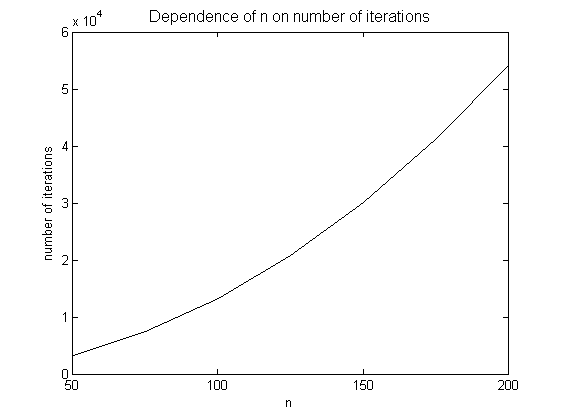
\includegraphics[width=1\linewidth]{figures/NumberOfIterations.png}
\end{minipage}%
\begin{minipage}{.5\textwidth}
  \centering
  \includegraphics[width=1\linewidth]{figures/NumberOfIterationsloglog.png}
\end{minipage}
\caption{The number of iterations of the while loop in the computed Jacobi method as a function of the number of steps $n$ plotted in both a normal graph and as a log-log plot. From the log-log plot it is evident that the number of iterations in the while loop is proportional to $n^2$, since the slope of the log-log plot is found to equal $2$.}
\label{fig:DependenceOnNumberOfIterations1}
\end{figure}
In the log-log plot, the relation is shown as a straight line with a slope of approximately $2$, which is calculated directly from the data for $n=100$ and $n=200$.
This yield that the number of iterations increases as the number of steps squared (that is, $n^2$), and hence an increment of $n$ has a great impact on the number of iteration. 
\fxnote{ikke sandt?}
E.g. with $n=100$ the number of iterations for the while loop in the Jacobi method is $13,200$, whilst when $n$ is doubled to $200$, the function runs through the while loop 54,071 times before the requirement of $max(a_{kl}^2) > \epsilon$ in \matref{eq:maxa} is fulfilled. 

The slowness of the Jacobi algorithm has the effect that it cannot be run for too large matrices, and hence there is a significant limit for how small the step length $h$ can be made, and ultimately a limit to the precision of the algorithm.  

It is, however, evident that the Jacobi method implemented in this project can be improved for solving the specific eigenvalue problem described by \matref{eq:NatureOfTheProblem5} and \eqref{eq:NatureOfTheProblem6} by taking into account that the matrix $\v{A}$ is tridiagonal and has constant values in the entrances adjacent to the diagonal.
\fxnote{reference ??} 
However, this improvement of the algorithm is not in the scope of this project.